\section{Field disposition}\label{sec:field-observer-shells}

\subsection{Observer-field}
\paragraph{Choice.}
In this note, a field is read as an observer-field: a retained closure structure whose memorum, regions, polychiral shell dressing, and boundaries carry returned-current orientation, duration, pressure, and closure state.

\subsection{Memorum}
The field's memorum is its retained predecessor closure, present boundary, and successor horizon. A field can contain finer fields. At the next enclosing address, the entire field can be bound as one monon cycle.

\subsection{Regions and boundaries}
\begin{definition}[Region]
A region is a declared retained part of a field. Regions carry current, closure, pressure, and returned-current orientation.
\end{definition}

\begin{definition}[Boundary]
A boundary is the retained interface of a declared region or field. Boundary accounting records current and closure across the boundary.
\end{definition}

\subsection{Polychiral shell dressing}
\begin{definition}[Polychiral shell dressing]
A polychiral shell dressing is field outer dressing. It carries alpha/Omega return orientation, polarization imbalance, return duration, pressure, and PADAR coupling.
\end{definition}

Tritrio::Tetratrio::hexon. \apref{app:cc-basic-shared-hexon}. Dimonhexon. \apref{app:cc-standalone-caged-names}.

\begin{figure}[H]
\centering
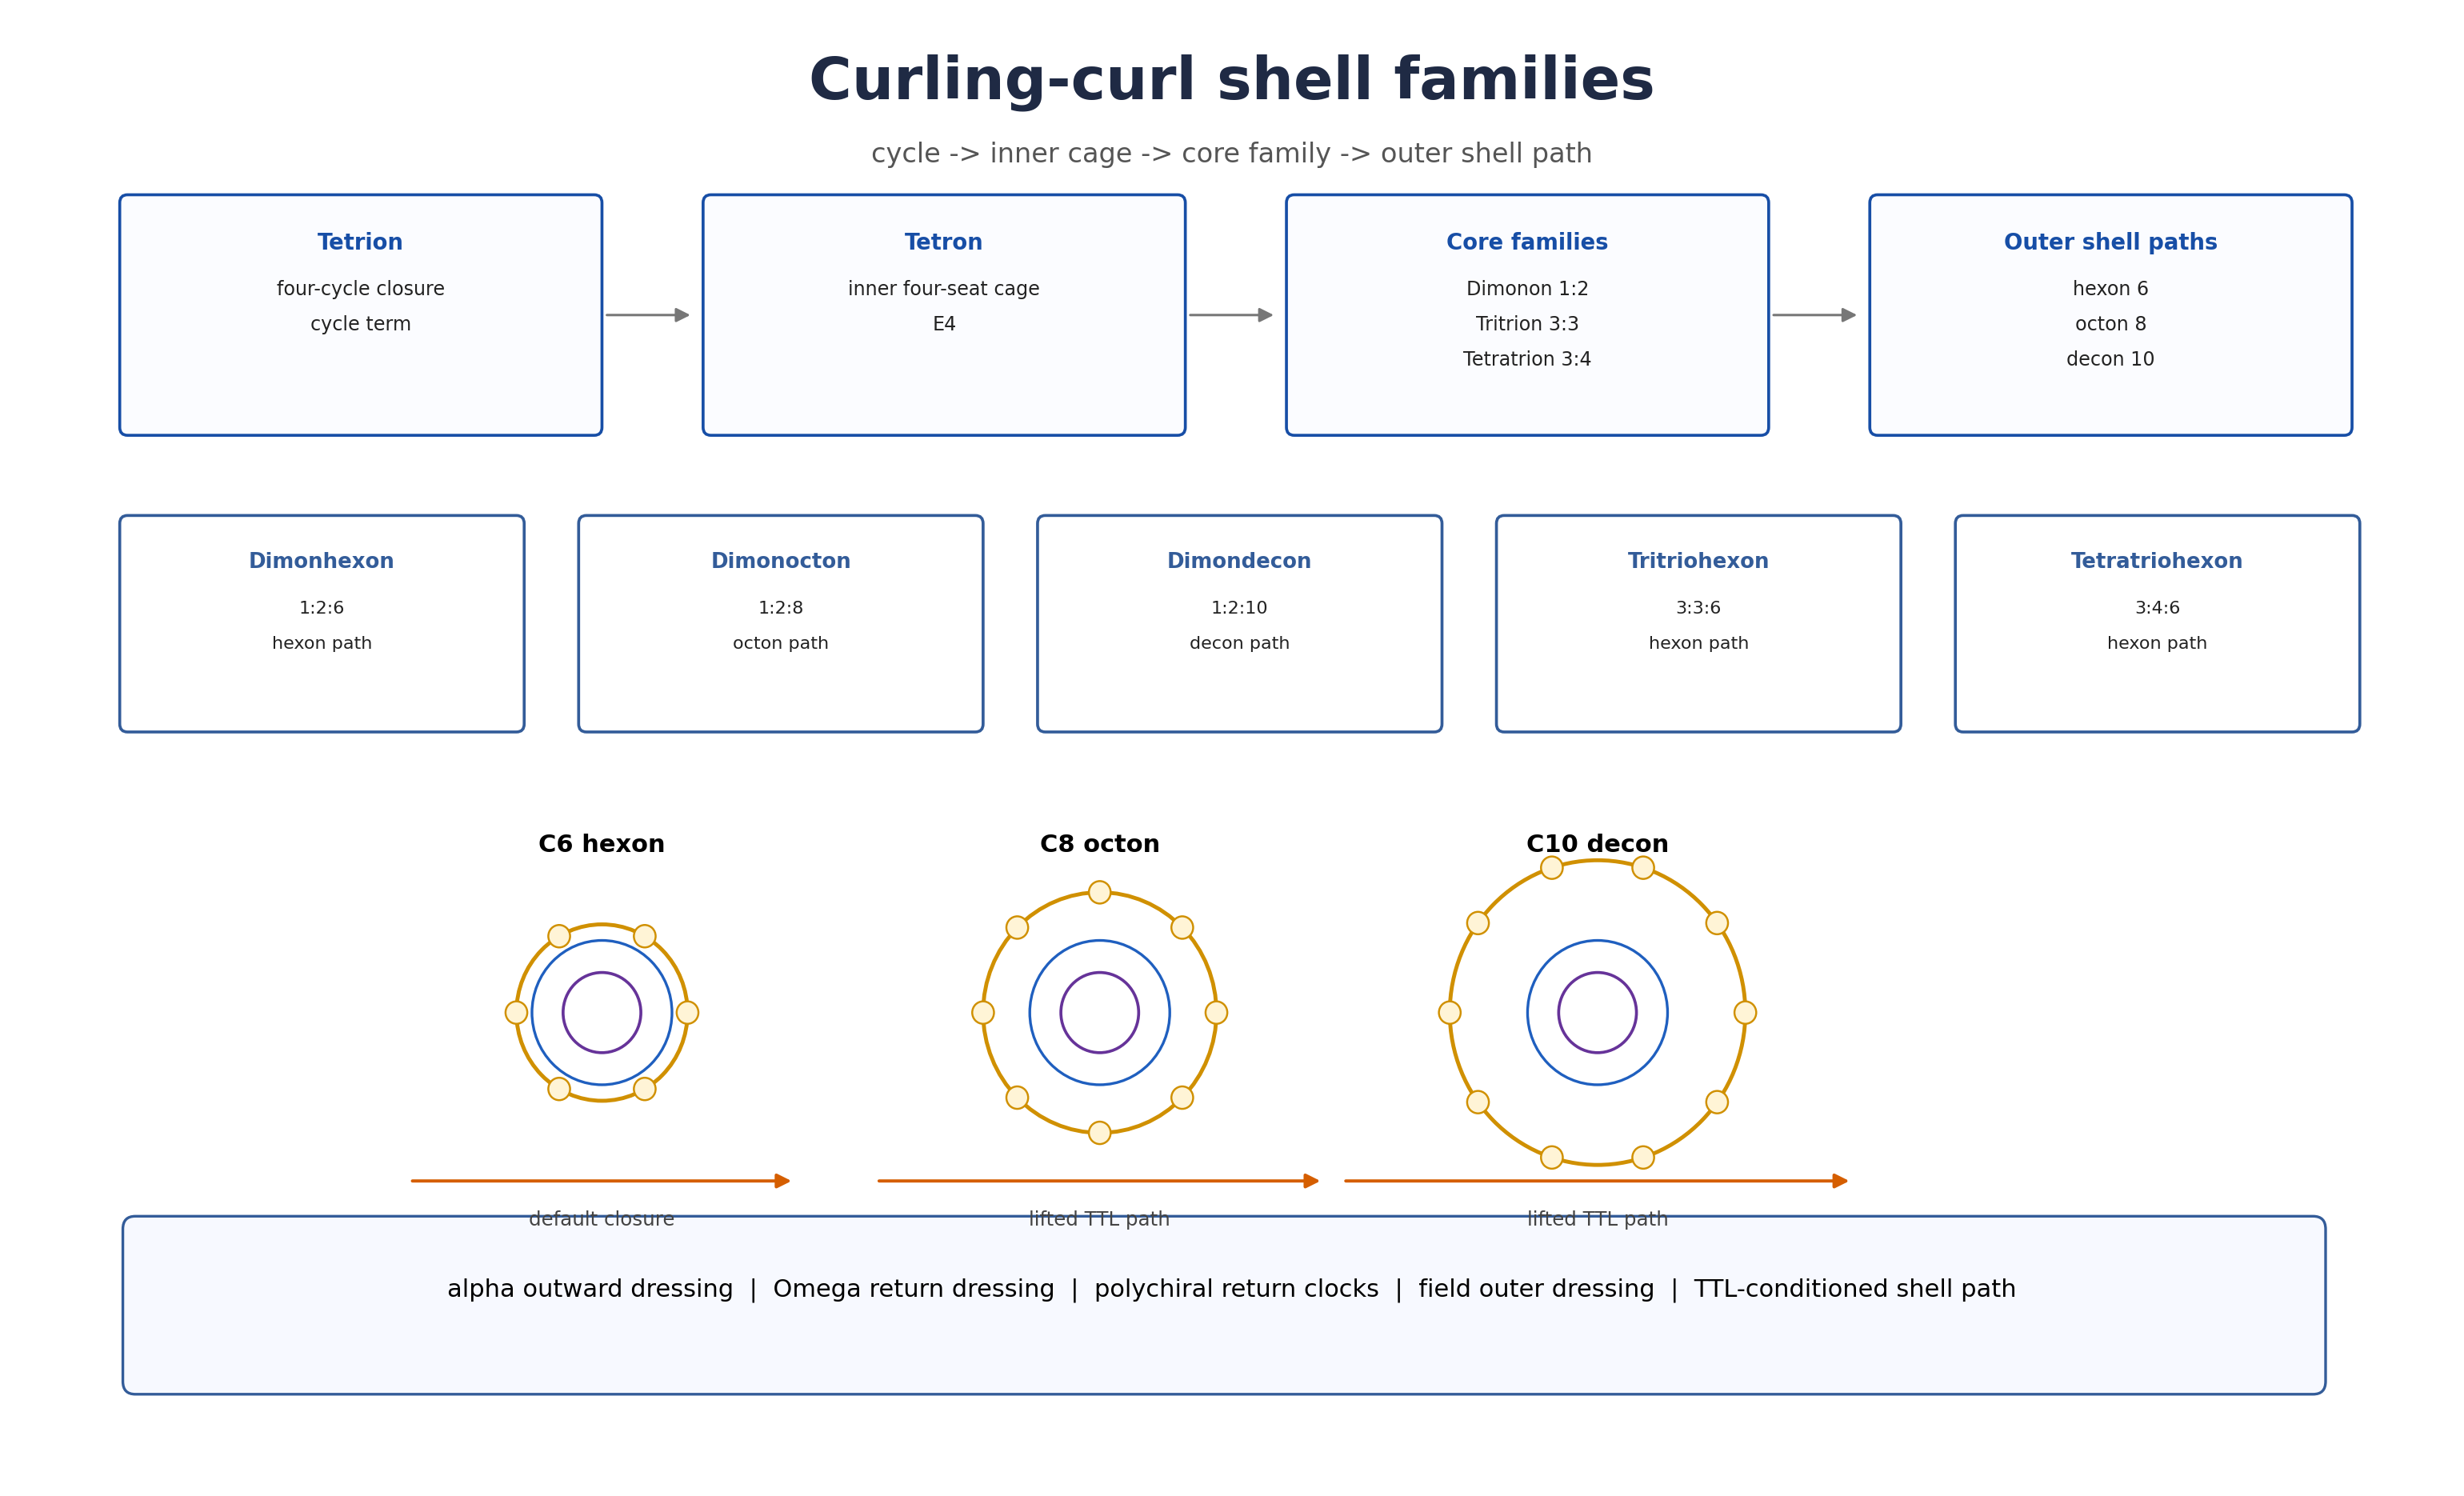
\includegraphics[width=0.96\linewidth]{figures_jpg/v39_15_curling_curl_layers.png}
\caption{Curling-curl shell families. Tetrion names the four-cycle closure; tetron names the default inner four-seat cage; Dimonon, Tritrion, and Tetratrion name core curling-curl families; hexon, octon, and decon name outer shell paths.}
\label{fig:curling-curl-shell-families}
\end{figure}

\subsection{Cage integrity}
\begin{definition}[Tetron]
A tetron is \(E_4\): the default inner cage with four seats. Hexon, octon, and decon name outer shell paths. \apref{app:cc-even-cages}.
\end{definition}

A boundary can cut through a retained cage for accounting. That partial boundary is a sample of the cage structure. The complete cage identity follows the retained even-address topology.

\paragraph{Channel count and shell burden.}
The occupied-seat count controls duon emission channels:
\[
N_{\mathrm{channels}}=\binom{\mathrm{occ}}{2}.
\]
The outer length \(L_{\mathrm{out}}\) controls shell-duration pressure burden. Occupancy and outer length remain distinct.
